\documentclass[12pt]{article}

\usepackage{graphicx}
\usepackage{amsmath}
\usepackage{amssymb}
\usepackage{natbib}
\usepackage{amsfonts}
\usepackage{multicol}
\usepackage{float}
\usepackage{oldgerm}
\usepackage{bm}
\usepackage{mathtools}
\usepackage{wrapfig}
\usepackage{fancyhdr}
\usepackage[export]{adjustbox}
\usepackage{xcolor}
\usepackage[shortlabels]{enumitem}

\pagestyle{empty}

\setlength{\headsep}{0.5cm}
\setlength{\oddsidemargin}{-0.5cm}
\setlength{\textwidth}{16.5cm}
\setlength{\textheight}{24cm}
\voffset = -2cm


\pagestyle{fancy}
\fancyhf{}
\rfoot{
\includegraphics[width=1.0in]{cnm.png}}
\lfoot{Homework 7}
\setlength\parindent{0pt}
\begin{document}

\begin{center}
\hfil
{\large\bf {ENGR 2910-101: Circuit Analysis}}
\hfill Instructor: Brian Rashap\\
Homework 7: 03/08/23 \hfill Due: 03/15/23\\
\hrulefill\\
\end{center}

{\bf Question 1} [10] % P6-03

The triangular pulse below is applied to a 20 mH inductor.

\begin{figure}[h!]
\begin{center}
 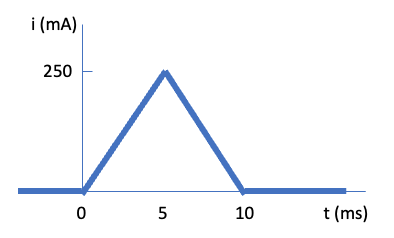
\includegraphics[scale=0.4]{fig6_3.png}
\end{center}
\end{figure}

\begin{enumerate}[(a)]
\item Write the expressions that describe $i(t)$ in the four intervals: \newline $t <0$, $0 \leq t \leq 5ms$, $5ms \leq t \leq 10ms$, $t> 10ms$.
\item Derive the expressions for the inductor, voltege, power, and energy. 
\end{enumerate}


\vspace{0.1in}

{\bf Question 2} [10] %P6-13

The voltage across a $5 \mu F$ capactior is know to be \newline

\begin{center}
$v_o = 500 t e^{-2500t} V$ for $t \geq 0$.
\end{center}

\begin{enumerate}[(a)]
\item Find the current through the capacitor for $t > 0$.
\item Find the power at the terminals of the capacitor when $t = 100 \mu s$.
\item Is the capacitor absorbing or delivering power at $t = 100 \mu s$.
\end{enumerate}

{\bf Question 3} [10] % P6-47

Two magnetically coupled coils are wound on a nonmagnetic core. The self-inductrance of coil 1 is $288 mH$, the mutual inductance is $90mH$, the coefficient of coupling is $0.75$, and the physical structure of the coils is such that $\mathcal{P}_{11} = \mathcal{P}_{22}$.

\begin{enumerate}[(a)]
\item Find $L_2$ and the turns ratio $\frac{N_1}{N_2}$.
\item If $N_1 = 1200$, what is the value of $\mathcal{P}_{1}$ and $\mathcal{P}_{2}$?
\end{enumerate} 

\newpage

{\bf Question 4 [10]} % P6-26

The two parallel inductors in the figure below are connected across the terminals of a black box at $t = 0$. The resulting voltage $v$ for $t>0$ is known to be $12 e^{-t} V$. It is also known that $i_1(0) = 2A$ and $i_2(0) = 4A$.

\begin{figure}[h!]
\begin{center}
 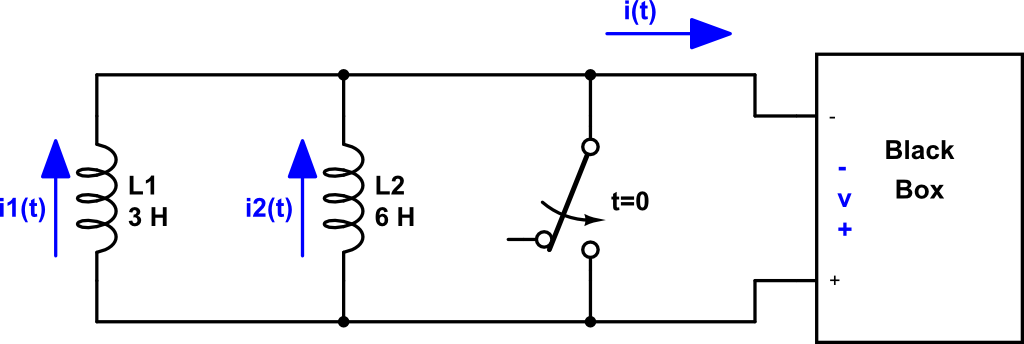
\includegraphics[scale=0.4]{p6_26.png}
\end{center}
\end{figure}

\begin{enumerate}[(a)]
\item Replace the original inductors with an euivalent inductor and find $i(t)$ for $t \geq 0$.
\item Find $i_1(t)$ for $t \geq 0$.
\item Find $i_2(t)$ for $t \geq 0$.
\item How much energy is delivered to the black box in the time interval $0 \leq t \leq \infty$.
\item How much energy was initially stored in the the parallel inducutors?
\item How much energy is trapped in the ideal inductors?
\item Show that your solutions for $i_1(t)$ and $i_2(t)$ agree with your answer in (f).
\end{enumerate} 

{\bf Question 5} [10] % P6_37

\begin{figure}[h!]
\begin{center}
 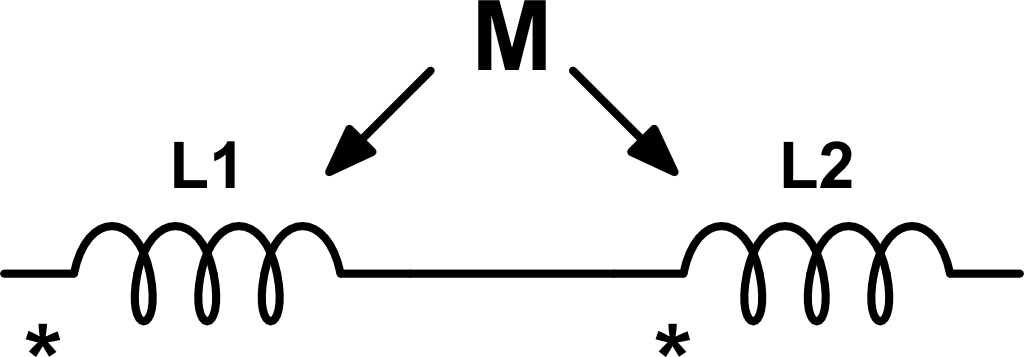
\includegraphics[scale=0.4]{p6_37.png}
\end{center}
\end{figure}

\begin{enumerate}[(a)]
\item Show that the two copled coils above can be replaced by a single coil having an inductance of $L_{ab} = L_a + L_b + 2M$. (\textit{Hint: express $v_{ab}$ in terms of $i_{ab}$.}
\item Show that if the connection to the terminals of the coil $L_2$ are reversed, then $L_{ab} = L_a + L_b - 2M$
\end{enumerate} 

\end{document}
